\setchapterpreamble[u]{\margintoc}
\chapter{Process Management}
\labch{procman}

\section{What are processes?}

\begin{definition}[Process]
  A process is an instance of a program that is being executed.
  It contains the program code and its current activity.
  Depending on the operating system (OS), a process may be made up of
  multiple threads of execution that execute instructions concurrently.
  Several processes may be associated with the same program; for example,
  opening up several instances of the same program often means more than
  one process is being executed.
  Each process has its own `process id` or \textbf{PID} to uniquely identify it.
\end{definition}

Whenever we run an application, or even a command on the linux shell, it spawns a process. Processes are always created by an already
existing process
\sidenote{
  Other than the very first process, which is always the
  \textbf{init} process. In most distributions, this is
  done by
  \href{https://systemd.io/}{systemd}, which is an
  init system that does a lot of other things as well.
  You can learn more about systemd and what all
  it does
  \href{https://documentation.suse.com/external-tree/en-us/sles/12-SP4/systemd\_in\_suse\_linux\_enterprise\_12\_white\_paper.pdf}{here}.
}
This creates a tree-like structure of processes, where each process has a parent process and can have multiple child processes.
When the parent of a process dies, the child processes are adopted by the \textbf{init} process.
\textbf{init} is thus the root of the process tree.

\begin{figure}[h!]
  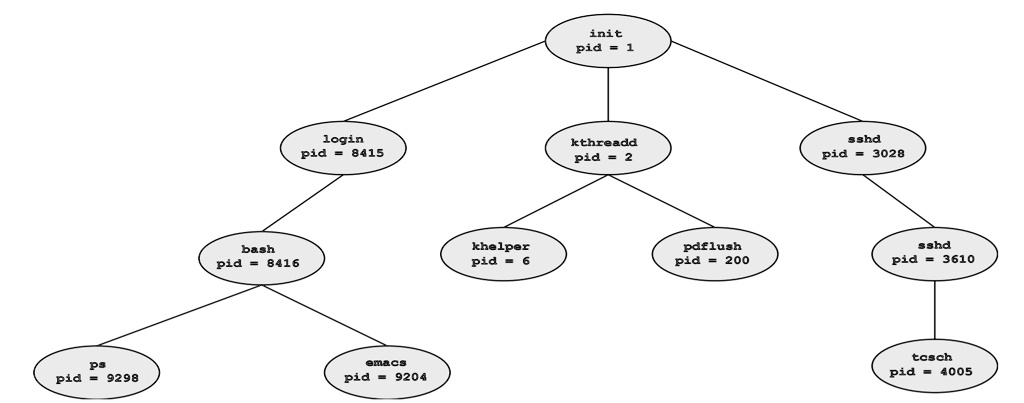
\includegraphics{process-tree}
  \caption{Example of a process tree}
  \labfig{process-tree}
\end{figure}

\begin{qs}
  How to get a snapshot of all the processes running?
  What are the commonly used flags used with it?
\end{qs}

\begin{ans}
  The \textbf{ps} command is used to get a snapshot of all the processes running.
  \begin{itemize}
    \item \textbf{ps} will get a snapshot of all the processes running.
    \item \textbf{ps -e} will show all the processes.
    \item \textbf{ps -f} will show full format listing.
    \item \textbf{ps -l} will show long format listing.
    \item \textbf{ps -u} will show user-oriented format listing.
    \item \textbf{ps -x} will show processes without controlling terminals.
    \item \textbf{ps -a} will show all processes with a terminal.
    \item \textbf{ps -A} will show all processes
    \item \textbf{ps aux} is a common command to see all processes
    \item \textbf{ps --forest} will show the processes in a tree form
  \end{itemize}
\end{ans}
